\section{Humans}
\Quote{Humans are fools, and hopelessly naive as well. They outnumber us; they are everywhere, and yet they have no more sense of their strength than a rat. Let us hope that the Datto remain that way.}{Dukkoti Nightrunner, elven warrior}

While not the strongest race, nor the quickest, humans have dominated the Tablelands for the last three thousand years.

\textbf{Personality:} More than other races, human personality is shaped by their social standing and background.

\begin{figure}[t!]
\centering
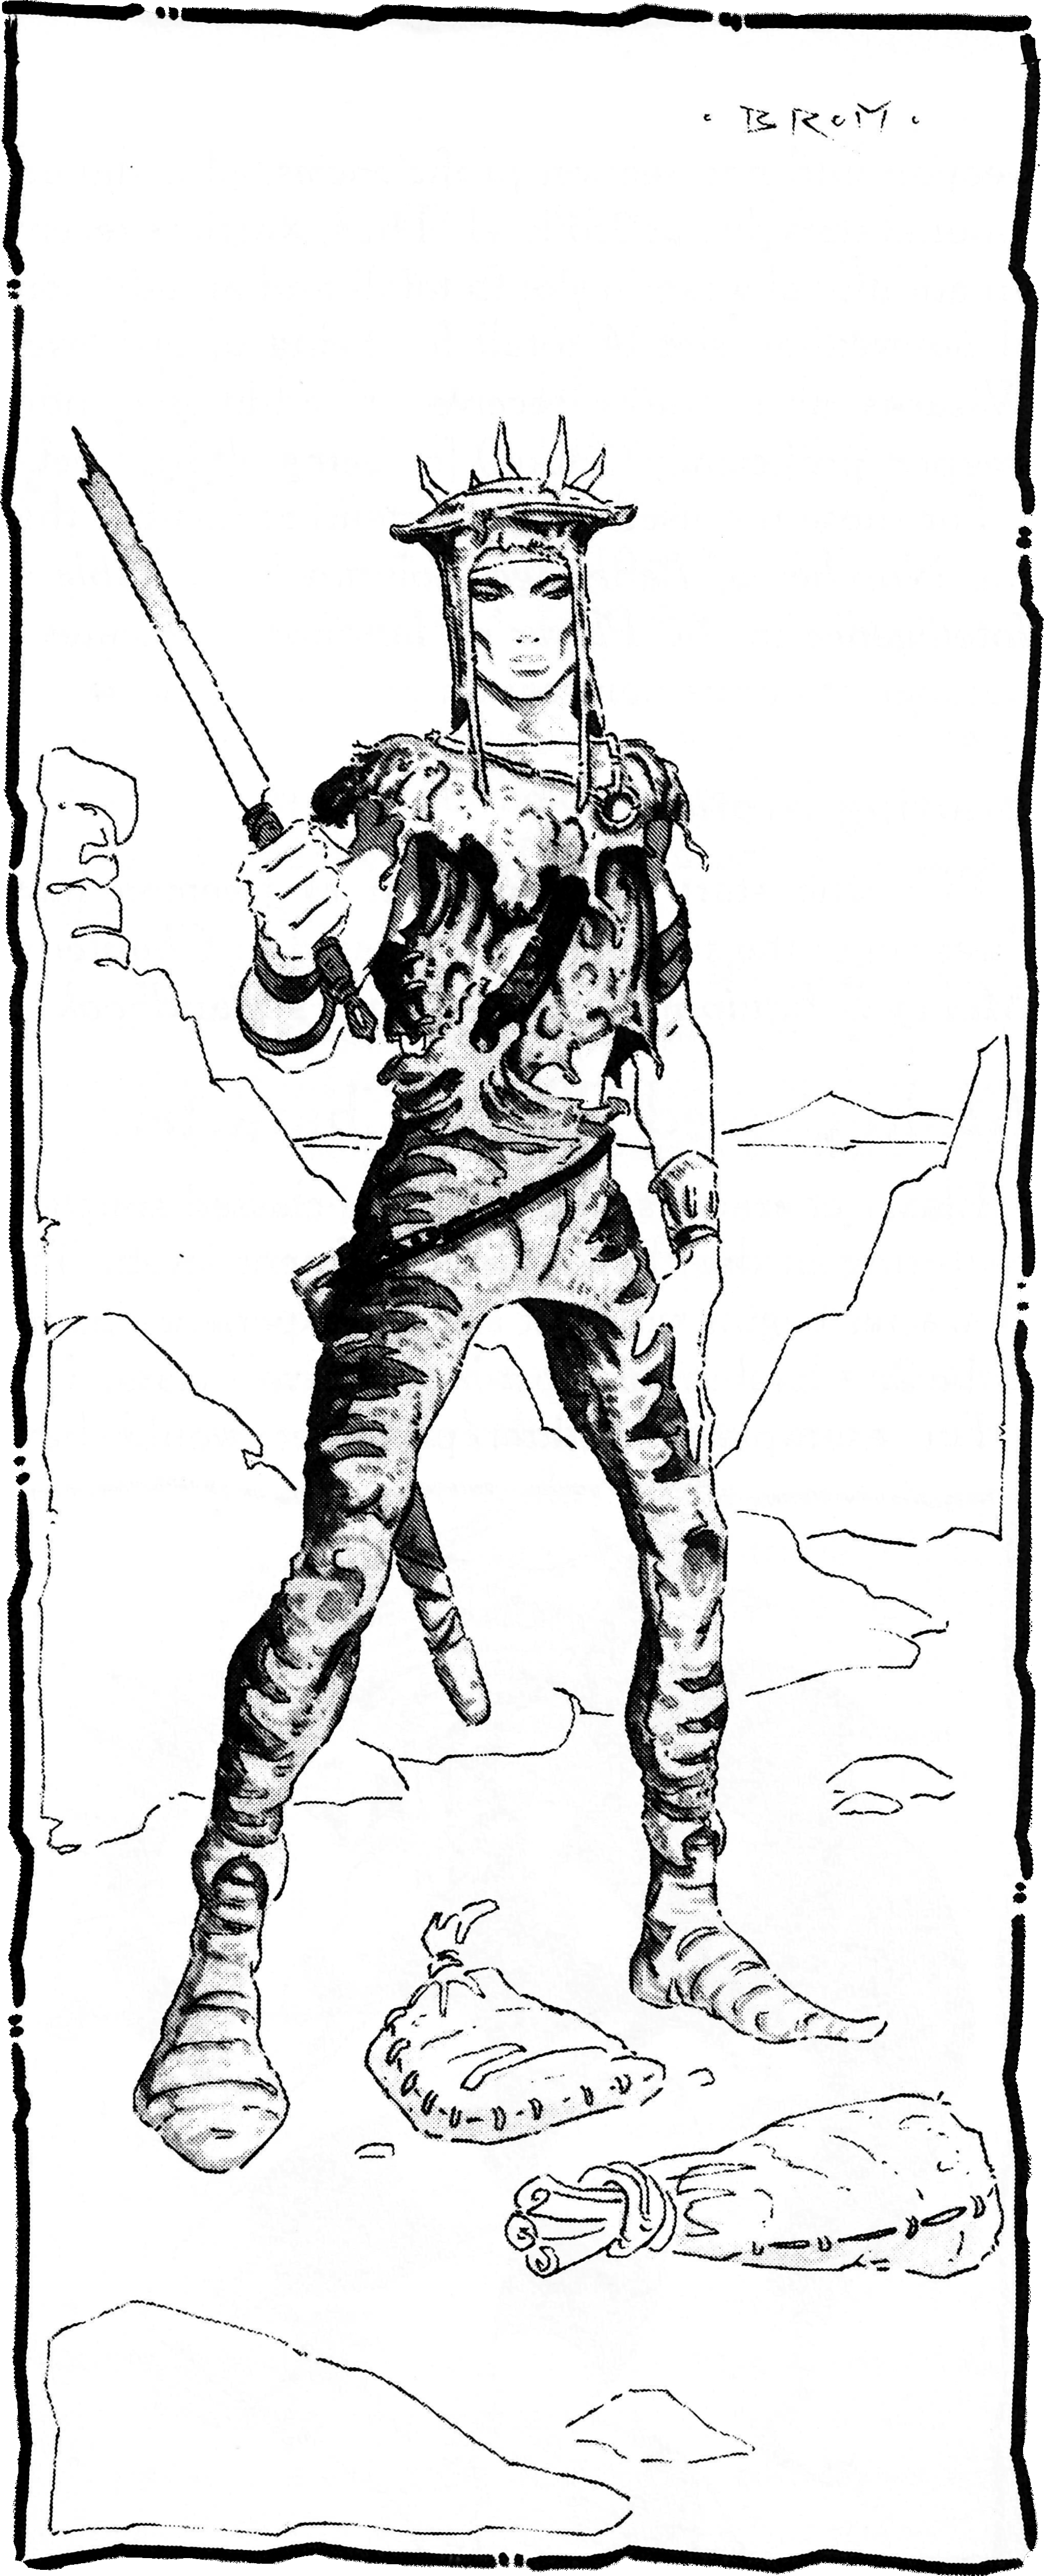
\includegraphics[width=\columnwidth]{images/human-1.png}
\WOTC
\end{figure}

\textbf{Physical Description:} Human males average 1.8 meter tall and 100 kg, while smaller females average 1.65 meters and 70 kg. Color of eyes, skin, and hair, and other physical features vary wildly; enlarged noses, webbed feet or extra digits are not uncommon.

\textbf{Relations:} Human treatment of other races is usually based on what their culture has taught them. In large settlements, such as in city-states, close proximity with many races leads to a suspicious unfriendly tolerance.

\textbf{Alignment:} Humans have no racial tendency toward any specific alignment.

\textbf{Human Lands:} Humans can be found anywhere, from the great city-states to the barren wastes.

\textbf{Magic:} Most humans fear and hate arcane magic, forming mobs to kill vulnerable wizards.

\textbf{Psionics:} Humans see the Way as a natural part of daily life, and readily become psions.

\textbf{Religion:} Most humans pay homage to the elements. Draji and Gulgs often worship their monarchs.

\textbf{Language:} Most humans speak the common tongue. Nobles and artisans within a given city-state usually speak the city language, but slaves typically only speak Common.

\textbf{Names:} Nobles, artisans and traders use titles or surnames; others some simply use one name.

\textbf{Male Names:} Agis of Asticles, King Tithian, Lord Vordon, Pavek, Trenbull Al'Raam'ke

\textbf{Female Names:} Akassia, General Zanthiros, Lady Essen of Rees, Neeva, Sadira

\textbf{Adventurers:} Some human adventurers seek treasure; others adventure for religious purposes as clerics or druids; others seek companionship or simply survival.

\subsection{Human Racial Traits}
\begin{itemize*}
  \item Medium: As Medium creatures, humans have no special bonuses or penalties due to their size. 
  \item Human base land speed is 9 meters.
  \item 1 extra feat at 1st level.
  \item 4 extra skill points at 1st level and 1 extra skill point at each additional level.
  \item Automatic Language: Common. Bonus Languages: Any (other than secret languages, such as Druidic). See the \skill{Speak Language} skill.
  \item Favored Class: Any. When determining whether a multiclass human takes an experience point penalty, his or her highest-level class does not count.
\end{itemize*}
